% Drawing 154/01-8 -- folder 154, batch 01, archive page 13 (PDF page 14).
% Transcription: figure : un arrangement de pseudo-droites orange, avec la droite jaune $D$ et une droite $\Delta$ qui la coupe en $a$ ; le secteur entre $D$ et $\Delta$ est hachuré au crayon, une flèche courbe va de $D$ vers $\Delta$
% Kind: pseudoline arrangement with a line D and a line Delta. Method 2 (schematic redraw from the facsimile). Status: ok.
% Notes: Seven orange pseudolines, the yellow line D, and the orange line Delta that cuts D at a (marked, one other orange line passes through a); the sectors between D and Delta hatched in pencil on both sides of a; a curved pencil arrow from D up to Delta; a grey pencil line. The label a is not legible on the facsimile; a marks the crossing as the transcription says.
% Coordinates: 1 unit = 1 mm = 1/100 of the crop width (bbox in page fractions: [0.483, 0.284, 0.782, 0.464]).
% Redrawn by Claude (claude-opus-5-5), issue #73, 2026-11-07; not checked by a human; not compiled (no TeX in the session).
% Revised by Claude (claude-opus-5-5) 2026-11-09 (issue #128) after Michel's check: vertices snapped to exact intersections (drawn points on their lines, meeting ends on the stroke they meet, near-concurrent lines through one computed point, curve ends on their rim); labels at \small as in folder 80 batch 3. Status: ok.
% Rights: reproduces part of the work -- behind RENDER_TRANSCRIPTS, never published by itself.
\documentclass[tikz,border=3pt]{standalone}
\usepackage{amsmath,amssymb}
\usetikzlibrary{patterns,arrows.meta}
\tikzset{Or/.style={orange!90!black}, Ye/.style={yellow!80!orange}, Lg/.style={green!60!black!70}, Dg/.style={green!45!black}, Br/.style={brown!80!black}, Rd/.style={red!85!black}, Bl/.style={blue!70!black}, Gy/.style={black!40}, pencil/.style={black!45}, struck/.style={black!35}, mark/.style={circle,draw,inner sep=1.3pt}, pt/.style={circle,fill,inner sep=0.9pt}, opt/.style={circle,draw,fill=white,inner sep=1.1pt}}
\begin{document}
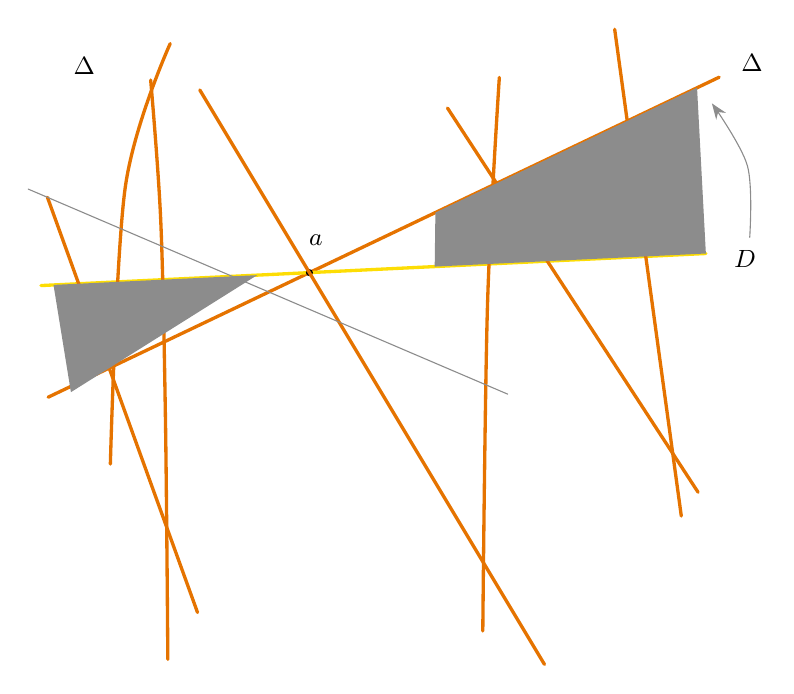
\begin{tikzpicture}[x=1mm,y=1mm,line cap=round,line join=round,font=\scriptsize]
\draw[Or,very thick] (5.4,-49.11) -- (90.62,-8.47);
\draw[Ye,very thick] (4.49,-34.93) -- (88.93,-30.86);
\node[pt] at (38.58,-33.29) {};
\node[inner sep=1pt] at (94.8,-6.7) {\small $\Delta$};
\node[inner sep=1pt] at (10,-7) {\small $\Delta$};
\node[inner sep=1pt] at (93.9,-31.5) {\small $D$};
\draw[Or,very thick] (5.31,-23.72) -- (24.37,-76.45);
\draw[Or,very thick] plot[smooth, tension=0.55] coordinates {(13.3,-57.6) (15.2,-22.4) (20.9,-4.2)};
\draw[Or,very thick] plot[smooth, tension=0.55] coordinates {(18.42,-8.83) (19.7,-26.7) (20.3,-52.1) (20.6,-82.4)};
\draw[Or,very thick] (24.66,-10.09) -- (68.43,-83.04);
\draw[Or,very thick] plot[smooth, tension=0.55] coordinates {(62.7,-8.5) (61.2,-37.3) (60.6,-78.8)};
\draw[Or,very thick] (56.12,-12.39) -- (87.94,-61.18);
\draw[Or,very thick] (77.35,-2.39) -- (85.81,-64.2);
\draw[pencil] (2.87,-22.68) -- (63.76,-48.72);
\fill[pattern=north east lines,pencil] (54.58,-25.66) -- (87.81,-9.8) -- (88.93,-30.86) -- (54.49,-32.52) -- cycle;
\fill[pattern=north east lines,pencil] (6.08,-34.85) -- (31.94,-33.61) -- (8.29,-48.47) -- cycle;
\draw[-{Stealth[length=2mm]},pencil] plot[smooth, tension=0.55] coordinates {(94.5,-28.8) (94.2,-19.7) (89.7,-11.8)};
\node[inner sep=1pt] at (39.4,-29.1) {\small $a$};
\end{tikzpicture}
\end{document}
